%!TEX root = main.tex

\subsection{The problem}

Find a best way to align two sequences including matches, substitutions and possible gaps.

\subsubsection{Gap penalties}

\begin{figure}[H]
	\centering
	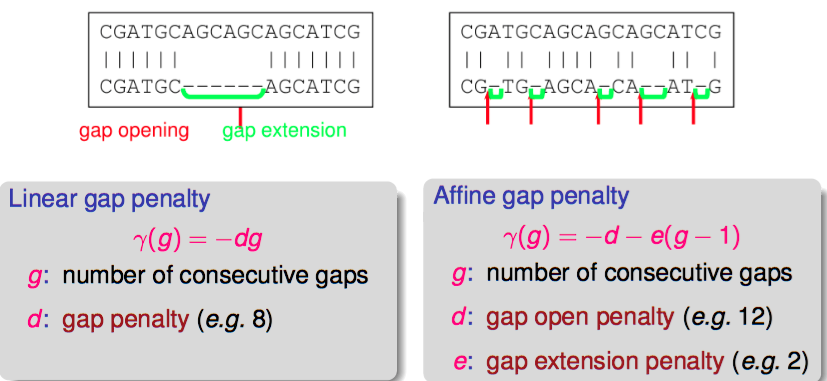
\includegraphics[scale=0.4]{images/09_gap.png}
 	\caption{Gap penalties. Afine is more relevant.}
\end{figure}

\subsubsection{Number of alignements}

The total number alignements is huge ($\frac{4^n}{\sqrt{\pi*n}}$). We need dynamic programming.

\begin{itemize}
	\item We look for maximal cumulative score;
	\item An optimal global alignment is made of optimal alignments between subsequences: decomposition of sub-problems computed only once.
\end{itemize}

\subsection{Global alignment: Needle-Wunsch}


\begin{figure}[htp]
	\centering
	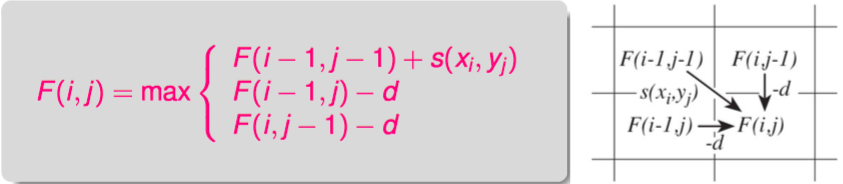
\includegraphics[scale=0.4]{images/10_global.png}
 	\caption{$F(n,m)$ is final alignment score. Need to follow backpointers. $O(n^2)$. }
\end{figure}


\subsection{Local alignment: Smith-Waterman}

\begin{figure}[htp]
	\centering
	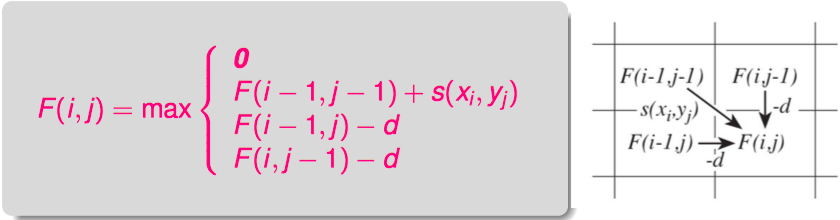
\includegraphics[scale=0.4]{images/11_local.png}
 	\caption{Find maximal $F(i,j)$ and follow backpointers till 0. Need negative scores for strong mismatches. $O(n^2)$.}
\end{figure}

\subsection{Variants}

\subsubsection{Semi-global alignment}
\begin{figure}[H]
	\centering
	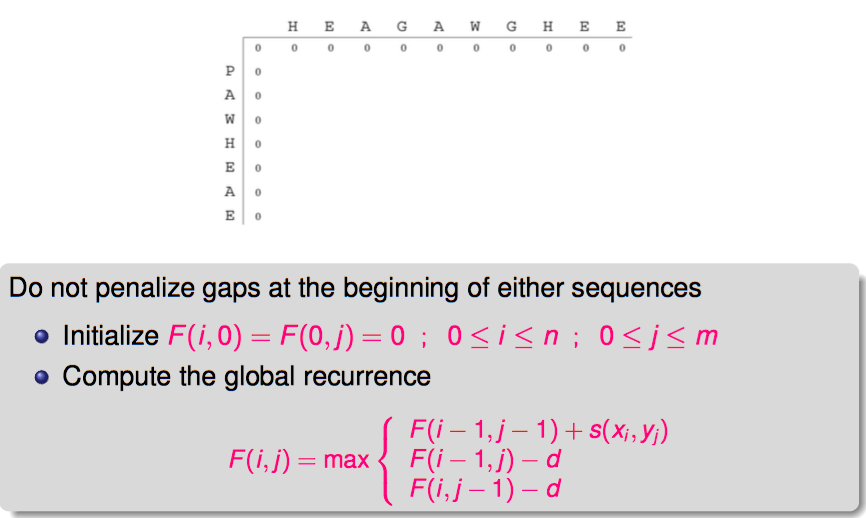
\includegraphics[scale=0.4]{images/12_semi.png}
\end{figure}

\subsubsection{Local alignment with repeats}


\begin{figure}[H]
	\centering
	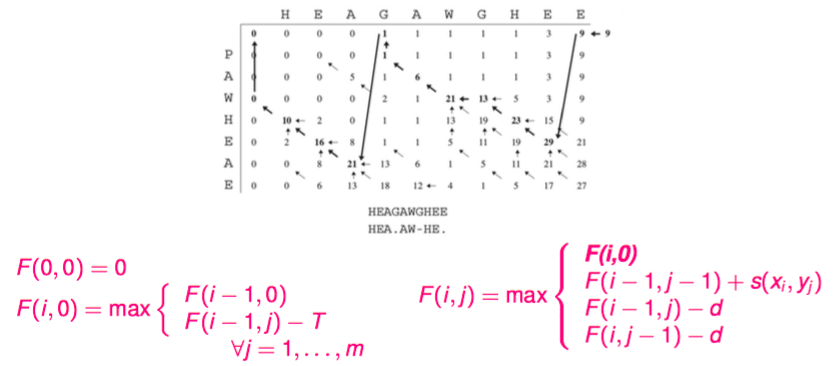
\includegraphics[scale=0.5]{images/13_repeats.png}
	\caption{Look for several matches (subsequences) of y into x. Scoring higher than T.}
\end{figure}

\subsubsection{Affine gap penalty}

\begin{figure}[H]
	\centering
	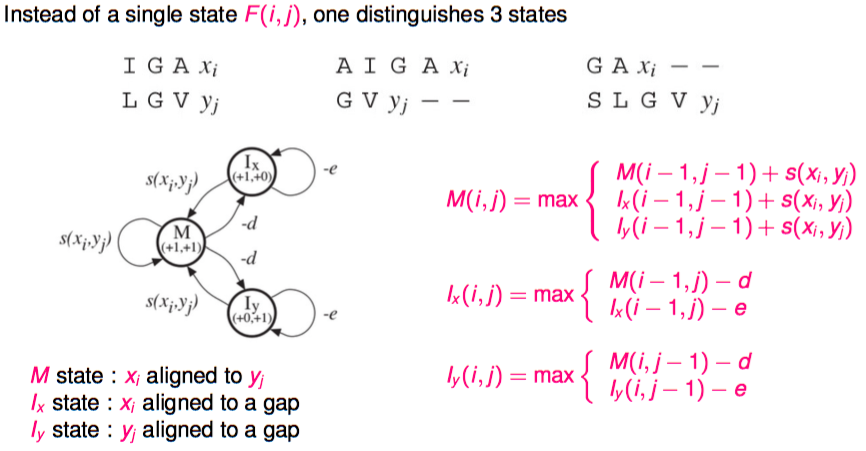
\includegraphics[scale=0.4]{images/14_affine.png}
\end{figure}

\subsection{Signifiance assessment}
\begin{figure}[htp]
	\centering
	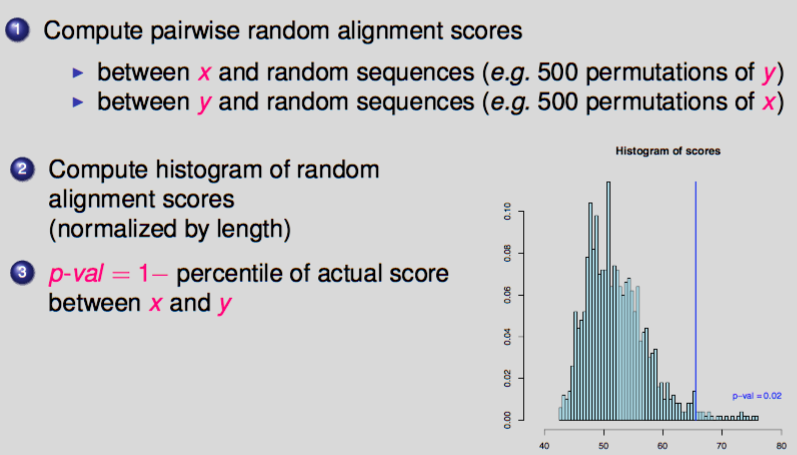
\includegraphics[scale=0.4]{images/15_procedure.png}
	\caption{Procedure.}
\end{figure}

The actual distribution of alginment scores is called \textbf{extreme value distribution}.

\begin{figure}[htp]
	\centering
	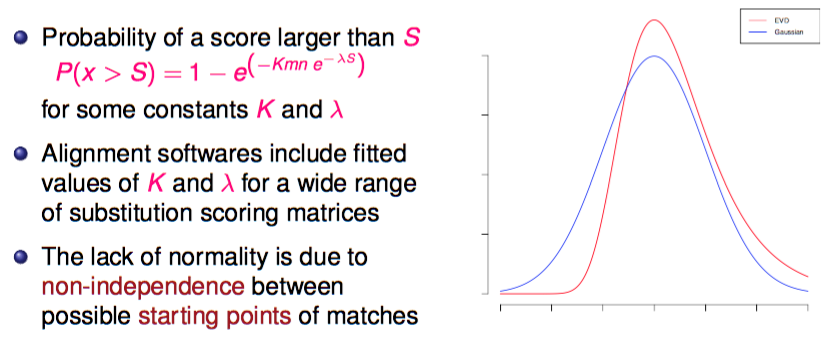
\includegraphics[scale=0.5]{images/16_evd.png}
	\caption{K is a multiplicative factor correcting non independance of possible starting poins for matches. $\lambda$ is a scale parameter.}
\end{figure}